\documentclass[a4paper]{article}
\usepackage[a4paper, margin=1in]{geometry} % Adjust margin here, e.g., 1 inch
% Some basic packages
\usepackage[utf8]{inputenc}
\usepackage[T1]{fontenc}
\usepackage{textcomp}
\usepackage[english]{babel}
\usepackage{url}
\usepackage{graphicx}
\usepackage{float}
\usepackage{booktabs}
% \usepackage{enumitem}
\usepackage{enumerate}
\usepackage[colorlinks]{hyperref}

\pdfminorversion=7

% Don't indent paragraphs, leave some space between them
\usepackage{parskip}
\usepackage{changepage}

% Hide page number when page is empty
\usepackage{emptypage}
\usepackage{subcaption}
\usepackage{multicol}
\usepackage[dvipsnames]{xcolor}

% Other font I sometimes use.
% \usepackage{cmbright}

% Math stuff
\usepackage{amsmath, amsfonts, mathtools, amsthm, amssymb}

% Add this line to make equation numbering follow section
\numberwithin{equation}{section}

% Fancy script capitals
\usepackage{mathrsfs}
\usepackage{cancel}
% Bold math
\usepackage{bm}
% Some shortcuts
\newcommand\N{\ensuremath{\mathbb{N}}}
\newcommand\R{\ensuremath{\mathbb{R}}}
\newcommand\Z{\ensuremath{\mathbb{Z}}}
\renewcommand\O{\ensuremath{\emptyset}}
\newcommand\Q{\ensuremath{\mathbb{Q}}}
\newcommand\C{\ensuremath{\mathbb{C}}}

% Easily typeset systems of equations (French package)
\usepackage{systeme}

% Put x \to \infty below \lim
\let\svlim\lim\def\lim{\svlim\limits}

%Make implies and impliedby shorter
\let\implies\Rightarrow
\let\impliedby\Leftarrow
\let\iff\Leftrightarrow
% \let\epsilon\varepsilon

% COURSE SPECIFICS
% GRIFFITHS
\ifdefined\pdfliteral
    \let\griffPdfliteral\pdfliteral
\else \def\griffPdfliteral#1{\special{pdf: literal #1}} \fi

\newcommand\griffr[1][2]{\leavevmode\hbox{\kern1pt\vbox to1ex{}\griffPdfliteral{%
    q 1 J .27 0 0 .27 0 0 cm #1 w
    0 2 m
    0 2 8.1 9.7 9.2 13.2 c
    10.4 16.8 8.4 15.4 8 14.7 c
    7.6 14 6.8 12.6 12 13 c
    17 13.5 14.5 7.8 13.7 6 c
    12.8 4.3 10.3 1.2 11.4 .2 c
    12.6 -.7 18.8 3.6 18.8 3.6 c
    18.8 3.6 l S Q
}\kern6pt}}
\newcommand\hatgriffr{\skew3\hat{\griffr[4]}}

% Add \contra symbol to denote contradiction
\usepackage{stmaryrd} % for \lightning
\newcommand\contra{\scalebox{1.5}{$\lightning$}}

% \let\phi\varphi

% Command for short corrections
% Usage: 1+1=\correct{3}{2}

\definecolor{correct}{HTML}{009900}
\newcommand\correct[2]{\ensuremath{\:}{\color{red}{#1}}\ensuremath{\to }{\color{correct}{#2}}\ensuremath{\:}}
\newcommand\green[1]{{\color{correct}{#1}}}

% horizontal rule
\newcommand\hr{
    \noindent\rule[0.5ex]{\linewidth}{0.5pt}
}

% hide parts
\newcommand\hide[1]{}

% si unitx
\usepackage{siunitx}
\sisetup{locale = FR}

% Environments
\makeatother
% For box around Definition, Theorem, ...
% \usepackage{mdframed}
\usepackage[framemethod=TikZ]{mdframed}

% Custom command to draw a rectangular border around an equation
\setlength{\fboxsep}{5pt}  % Adjust padding inside the box
\usepackage{empheq}
\newcommand*\widefbox[1]{\fbox{\hspace{1em}#1\hspace{1em}}}

\usepackage{environ}  % This package allows for easier custom environment definitions

% Define the custom environment
\NewEnviron{framed}{%
  \begin{empheq}[box=\fbox]{align}
  \BODY
  \end{empheq}
}
% Custom environment to box align equations
% \newenvironment{boxedalign}
%   {\begin{empheq}[box=\fbox]{align}}
%   {\end{align}\end{empheq}}

\newtheorem{thm}{Theorem}[subsection]
\newtheorem{defi}[thm]{Definition}
\newtheorem{lem}[thm]{Lemma}
\newtheorem{ret}{Correction}


\newtheorem*{term}{Terminology}
\newtheorem*{key}{Keywords and Related Concepts}
\newtheorem{lign}[thm]{Equation}
\newtheorem{law}[thm]{Law / Principle}

\usepackage{mathtools}
\DeclarePairedDelimiter\bra{\langle}{\rvert}
\DeclarePairedDelimiter\ket{\lvert}{\rangle}
\DeclarePairedDelimiterX\braket[2]{\langle}{\rangle}{#1\,\delimsize\vert\,\mathopen{}#2}


% \newcounter{theo}[section]
% \renewcommand{\thetheo}{\arabic{section}.\arabic{theo}}

% \mdfsetup{skipabove=1em,skipbelow=0em}
% \theoremstyle{definition}
% \newmdtheoremenv[nobreak=true]{definition}{Definition}
% \newmdtheoremenv[nobreak=true]{theorem}{Theorem}
% \newmdtheoremenv[nobreak=true]{corollary}{Corollary}
% \newmdtheoremenv[nobreak=true]{lemma}{Lemma}

% \newtheorem*{observation}{Observation}
% \newtheorem*{property}{Property}
% \newtheorem*{postulate}{Postulate}
% \newtheorem*{conclusion}{Conlusion}
% \newtheorem*{repitition}{Repitition}
% \newtheorem*{example}{Example}
% \newtheorem*{question}{Question}
% \newtheorem*{intuition}{Intuition}

% End example and intermezzo environments with a small diamond (just like proof
% environments end with a small square)
% \usepackage{etoolbox}
% \AtEndEnvironment{example}{\null\hfill$\diamond$}%
% \AtEndEnvironment{repitition}{\null\hfill$\diamond$}%
% \AtEndEnvironment{opmerking}{\null\hfill$\diamond$}%

% Fix some spacing
% http://tex.stackexchange.com/questions/22119/how-can-i-change-the-spacing-before-theorems-with-amsthm
\makeatletter
\def\thm@space@setup{%
  \thm@preskip=\parskip \thm@postskip=0pt
}


% Exercise 
% Usage:
% \oefening{5}
% \suboefening{1}
% \suboefening{2}
% \suboefening{3}
% gives
% Oefening 5
%   Oefening 5.1
%   Oefening 5.2
%   Oefening 5.3
\newcommand{\exercise}[1]{%
    \def\@exercise{#1}%
    \subsection*{Exercise #1}
}

\newcommand{\subexercise}[1]{%
    \subsubsection*{Exercise \@exercise.#1}
}

\usepackage{xcolor}
\newcommand{\textred}[1]{\textcolor{red}{#1}}

% \lecture starts a new lecture (les in dutch)
%
% Usage:
% \lecture{1}{di 12 feb 2019 16:00}{Inleiding}
%
% This adds a section heading with the number / title of the lecture and a
% margin paragraph with the date.

% I use \dateparts here to hide the year (2019). This way, I can easily parse
% the date of each lecture unambiguously while still having a human-friendly
% short format printed to the pdf.

\usepackage{xifthen}
\def\testdateparts#1{\dateparts#1\relax}
\def\dateparts#1 #2 #3 #4 #5\relax{
    \marginpar{\small\textsf{\mbox{#1 #2 #3 #5}}}
}

\def\@lecture{}%
\newcommand{\lecture}[3]{
    \ifthenelse{\isempty{#3}}{%
        \def\@lecture{Lecture #1}%
    }{%
        \def\@lecture{Lecture #1: #3}%
    }%
    \subsection*{\@lecture}
    \marginpar{\small\textsf{\mbox{#2}}}
}

\def\@chapter{}%
\newcommand{\chapter}[3]{
    \ifthenelse{\isempty{#3}}{%
        \def\@chapter{Chapter #1}%
    }{%
        \def\@chapter{Chapter #1: #3}%
    }%
    \subsection*{\@chapter}
    \marginpar{\small\textsf{\mbox{#2}}}
}

\def\@week{}%
\newcommand{\week}[3]{
    \ifthenelse{\isempty{#3}}{%
        \def\@week{Uge #1}%
    }{%
        \def\@week{Uge #1: #3}%
    }%
    \subsection*{\@week}
    \marginpar{\small\textsf{\mbox{#2}}}
}

% These are the fancy headers
% \usepackage{fancyhdr}
% \pagestyle{fancy}

% LE: left even
% RO: right odd
% CE, CO: center even, center odd
% My name for when I print my lecture notes to use for an open book exam.
% \fancyhead[LE,RO]{Gilles Castel}

% \setlength{\headheight}{5pt}

% % \fancyhead[R]{\@lecture} % Right odd,  Left even
% \fancyfoot[R]{\thepage}  % Right odd,  Left even
% \fancyfoot[C]{\leftmark}     % Center

\makeatother

% Todonotes and inline notes in fancy boxes
\usepackage{todonotes}
\usepackage{tcolorbox}

% Make boxes breakable
\tcbuselibrary{breakable}

% Usage: 
% \begin{correction}
%     Lorem ipsum dolor sit amet, consetetur sadipscing elitr, sed diam nonumy eirmod
%     tempor invidunt ut labore et dolore magna aliquyam erat, sed diam voluptua. At
%     vero eos et accusam et justo duo dolores et ea rebum. Stet clita kasd gubergren,
%     no sea takimata sanctus est Lorem ipsum dolor sit amet.
% \end{correction}
\newenvironment{correction}{\begin{tcolorbox}[
    arc=0mm,
    colback=white,
    colframe=green!60!black,
    title=Correction,
    fonttitle=\sffamily,
    breakable
]}{\end{tcolorbox}}

% Same as 'correction' but color of box is different
\newenvironment{note}{\begin{tcolorbox}[
    arc=0mm,
    colback=white,
    colframe=white!60!black,
    title=Note,
    fonttitle=\sffamily,
    breakable
]}{\end{tcolorbox}}


% Figure support as explained in my blog post.
\usepackage{import}
\usepackage{xifthen}
\usepackage{pdfpages}
\usepackage{transparent}
\newcommand{\incfig}[1]{%
    \def\svgwidth{\columnwidth}
    \import{./figures/}{#1.pdf_tex}
}

% Fix some stuff
% %http://tex.stackexchange.com/questions/76273/multiple-pdfs-with-page-group-included-in-a-single-page-warning
\pdfsuppresswarningpagegroup=1


% My name
\author{Erik Bach Ryhl}


\graphicspath{ {./figs/} }

\setcounter{tocdepth}{4}
\setcounter{secnumdepth}{3}

\title{Electromagnetism}
\begin{document}
    \maketitle
    \tableofcontents
    \newpage

    \section{Basics of Electromagnetism - A Quick Recap of The Static Theories}
    \subsection{The Electric Field}
    % Coloumb's Law
    % Superposition
    \subsubsection{Divergence and Curl of the Electric Field}
    \subsubsection{Boundary Conditions}
    \subsubsection{Conductors and Capacitors}
    \subsection{Potentials}
    \subsubsection{Laplace's Equation}
    \subsubsection{Uniqueness Theorem}
    \subsubsection{Multipole Expansion and Dipoles}
    \subsection{Electric Fields in Matter}
    \subsubsection{Forces and Torque}
    \subsubsection{Linear Dielectrics and the Displacement Field}
    \subsection{The Magnetic Field}
    % Lorent'z Force Law
    % Biot-Savart Law
    \subsubsection{Divergence and Curl of the Magnetic Field}
    \subsubsection{Boundary Conditions}
    \subsubsection{The Magnetic Vector Potential}
    \paragraph{Magnetic Dipoles}
    \subsection{Magnetic Fields in Matter}
    \subsubsection{Forces and Torque}
    \subsubsection{Paramagnatism vs. Diamagnatism}
    \subsubsection{Linear Media and the Auxiliary Field}
    \subsection{Electrodynamics}
    \subsubsection{Ohm's Law}
    \subsubsection{The Electromotive Force}
    \subsubsection{Faraday's Law}
    \subsubsection{Overview and What's Next}

    \section{Electromagnetism 2}
    \subsection{Conservation theorems}

    \textbf{Poynting's vector} 
    \begin{align*}
        \frac{dW}{dt} = \int_V d \tau \mathbf{E} \cdot \mathbf{J} &= \int_V d \tau \mathbf{E} \cdot \left( \frac{1}{\mu_0} \nabla \times \mathbf{B} - \epsilon_0 \frac{\partial \mathbf{E}}{\partial t}\right) \\
        &= \int _V d \tau \left( \frac{1}{\mu _0} E_i \epsilon_{ijk} \partial_j B_k - \frac{\epsilon_0}{2} \frac{\partial E^{2} }{\partial t} \right) \\
        &= \int _V d \tau \left( \frac{1}{\mu _0}E_i\epsilon _{jki}\partial _j B_k  -  \frac{\epsilon_0}{2} \frac{\partial E^{2} }{\partial t}\right) \\
        &= \int _V d \tau \left( \frac{1}{\mu _0}\epsilon _{jki} \partial _j B_k E_i - \frac{1}{\mu _0} \epsilon_{jki} B_k\partial_j E_i - \frac{1}{\mu _0}  -  \frac{\epsilon_0}{2} \frac{\partial E^{2} }{\partial t}\right)\\
        &= \int _V d \tau \left( \frac{1}{\mu _0} \nabla \cdot (\mathbf{B} \times \mathbf{E}) + \frac{1}{\mu _0} \mathbf{B}\cdot (\nabla \times \mathbf{E})  -  \frac{\epsilon_0}{2} \frac{\partial E^{2} }{\partial t}\right)\\
        &= \int _V d \tau \left( \frac{1}{\mu _0} \nabla \cdot (\mathbf{B} \times \mathbf{E}) - \frac{1}{2\mu _0} \frac{\partial B^{2} }{\partial t}   -  \frac{\epsilon_0}{2} \frac{\partial E^{2} }{\partial t}\right)\\
        &= - \frac{d}{dt} \int_V d \tau \left( \frac{1}{2\mu _0} B^{2} + \frac{\epsilon_0}{2} E^{2}  \right) - \frac{1}{\mu _0}\oint_S \left(\mathbf{E} \times \mathbf{B} \right)  \cdot d \mathbf{a}
    \end{align*}
    The integrand in the first term if the total electromagnetic field energy per unit volume \begin{align*}
        u \equiv \frac{1}{2 \mu _0} B^{2}  + \frac{\epsilon_0}{2} E^{2} 
    \end{align*}
    and the second term is called \textbf{Poynting's vector} \begin{align*}
        \boxed{\mathbf{S} \equiv \frac{1}{\mu_0} \left(\mathbf{E} \times \mathbf{B} \right)}
    \end{align*} 

    If there are no charges in the volume we are considering, then there is nothing to do work on, and hence \(dW / dt = 0\). Then 
    \begin{align*}
        \frac{d}{dt} \int_V d \tau \left( \frac{1}{2\mu _0} B^{2} + \frac{\epsilon_0}{2} E^{2}  \right) = - \int_V d \tau \left(\nabla \cdot \mathbf{S}\right) \implies \frac{\partial u}{\partial t} + \nabla \cdot \mathbf{S} = 0
    \end{align*}
    Thus the \textbf{continuity equation for energy in the fields} reads \begin{align*}
        \boxed{\frac{\partial u}{\partial t} + \nabla \cdot \mathbf{S} = 0} 
    \end{align*}
    which clearly shows that \(\mathbf{S}\) can be interpreted as energy flux of the fields through a given surface. The fact that it also is this way for non-closed surfaces is directly seen from the differential version of the continuity equation above, and it is thanks to the divergence theorem that we get the local differential version independent of surfaces.
    
    \newpage
    \documentclass[a4paper]{article}
\usepackage[a4paper, margin=1in]{geometry} % Adjust margin here, e.g., 1 inch
% Some basic packages
\usepackage[utf8]{inputenc}
\usepackage[T1]{fontenc}
\usepackage{textcomp}
\usepackage[english]{babel}
\usepackage{url}
\usepackage{graphicx}
\usepackage{float}
\usepackage{booktabs}
% \usepackage{enumitem}
\usepackage{enumerate}
\usepackage[colorlinks]{hyperref}

\pdfminorversion=7

% Don't indent paragraphs, leave some space between them
\usepackage{parskip}
\usepackage{changepage}

% Hide page number when page is empty
\usepackage{emptypage}
\usepackage{subcaption}
\usepackage{multicol}
\usepackage[dvipsnames]{xcolor}

% Other font I sometimes use.
% \usepackage{cmbright}

% Math stuff
\usepackage{amsmath, amsfonts, mathtools, amsthm, amssymb}

% Add this line to make equation numbering follow section
\numberwithin{equation}{section}

% Fancy script capitals
\usepackage{mathrsfs}
\usepackage{cancel}
% Bold math
\usepackage{bm}
% Some shortcuts
\newcommand\N{\ensuremath{\mathbb{N}}}
\newcommand\R{\ensuremath{\mathbb{R}}}
\newcommand\Z{\ensuremath{\mathbb{Z}}}
\renewcommand\O{\ensuremath{\emptyset}}
\newcommand\Q{\ensuremath{\mathbb{Q}}}
\newcommand\C{\ensuremath{\mathbb{C}}}

% Easily typeset systems of equations (French package)
\usepackage{systeme}

% Put x \to \infty below \lim
\let\svlim\lim\def\lim{\svlim\limits}

%Make implies and impliedby shorter
\let\implies\Rightarrow
\let\impliedby\Leftarrow
\let\iff\Leftrightarrow
% \let\epsilon\varepsilon

% COURSE SPECIFICS
% GRIFFITHS
\ifdefined\pdfliteral
    \let\griffPdfliteral\pdfliteral
\else \def\griffPdfliteral#1{\special{pdf: literal #1}} \fi

\newcommand\griffr[1][2]{\leavevmode\hbox{\kern1pt\vbox to1ex{}\griffPdfliteral{%
    q 1 J .27 0 0 .27 0 0 cm #1 w
    0 2 m
    0 2 8.1 9.7 9.2 13.2 c
    10.4 16.8 8.4 15.4 8 14.7 c
    7.6 14 6.8 12.6 12 13 c
    17 13.5 14.5 7.8 13.7 6 c
    12.8 4.3 10.3 1.2 11.4 .2 c
    12.6 -.7 18.8 3.6 18.8 3.6 c
    18.8 3.6 l S Q
}\kern6pt}}
\newcommand\hatgriffr{\skew3\hat{\griffr[4]}}

% Add \contra symbol to denote contradiction
\usepackage{stmaryrd} % for \lightning
\newcommand\contra{\scalebox{1.5}{$\lightning$}}

% \let\phi\varphi

% Command for short corrections
% Usage: 1+1=\correct{3}{2}

\definecolor{correct}{HTML}{009900}
\newcommand\correct[2]{\ensuremath{\:}{\color{red}{#1}}\ensuremath{\to }{\color{correct}{#2}}\ensuremath{\:}}
\newcommand\green[1]{{\color{correct}{#1}}}

% horizontal rule
\newcommand\hr{
    \noindent\rule[0.5ex]{\linewidth}{0.5pt}
}

% hide parts
\newcommand\hide[1]{}

% si unitx
\usepackage{siunitx}
\sisetup{locale = FR}

% Environments
\makeatother
% For box around Definition, Theorem, ...
% \usepackage{mdframed}
\usepackage[framemethod=TikZ]{mdframed}

% Custom command to draw a rectangular border around an equation
\setlength{\fboxsep}{5pt}  % Adjust padding inside the box
\usepackage{empheq}
\newcommand*\widefbox[1]{\fbox{\hspace{1em}#1\hspace{1em}}}

\usepackage{environ}  % This package allows for easier custom environment definitions

% Define the custom environment
\NewEnviron{framed}{%
  \begin{empheq}[box=\fbox]{align}
  \BODY
  \end{empheq}
}
% Custom environment to box align equations
% \newenvironment{boxedalign}
%   {\begin{empheq}[box=\fbox]{align}}
%   {\end{align}\end{empheq}}

\newtheorem{thm}{Theorem}[subsection]
\newtheorem{defi}[thm]{Definition}
\newtheorem{lem}[thm]{Lemma}
\newtheorem{ret}{Correction}


\newtheorem*{term}{Terminology}
\newtheorem*{key}{Keywords and Related Concepts}
\newtheorem{lign}[thm]{Equation}
\newtheorem{law}[thm]{Law / Principle}

\usepackage{mathtools}
\DeclarePairedDelimiter\bra{\langle}{\rvert}
\DeclarePairedDelimiter\ket{\lvert}{\rangle}
\DeclarePairedDelimiterX\braket[2]{\langle}{\rangle}{#1\,\delimsize\vert\,\mathopen{}#2}


% \newcounter{theo}[section]
% \renewcommand{\thetheo}{\arabic{section}.\arabic{theo}}

% \mdfsetup{skipabove=1em,skipbelow=0em}
% \theoremstyle{definition}
% \newmdtheoremenv[nobreak=true]{definition}{Definition}
% \newmdtheoremenv[nobreak=true]{theorem}{Theorem}
% \newmdtheoremenv[nobreak=true]{corollary}{Corollary}
% \newmdtheoremenv[nobreak=true]{lemma}{Lemma}

% \newtheorem*{observation}{Observation}
% \newtheorem*{property}{Property}
% \newtheorem*{postulate}{Postulate}
% \newtheorem*{conclusion}{Conlusion}
% \newtheorem*{repitition}{Repitition}
% \newtheorem*{example}{Example}
% \newtheorem*{question}{Question}
% \newtheorem*{intuition}{Intuition}

% End example and intermezzo environments with a small diamond (just like proof
% environments end with a small square)
% \usepackage{etoolbox}
% \AtEndEnvironment{example}{\null\hfill$\diamond$}%
% \AtEndEnvironment{repitition}{\null\hfill$\diamond$}%
% \AtEndEnvironment{opmerking}{\null\hfill$\diamond$}%

% Fix some spacing
% http://tex.stackexchange.com/questions/22119/how-can-i-change-the-spacing-before-theorems-with-amsthm
\makeatletter
\def\thm@space@setup{%
  \thm@preskip=\parskip \thm@postskip=0pt
}


% Exercise 
% Usage:
% \oefening{5}
% \suboefening{1}
% \suboefening{2}
% \suboefening{3}
% gives
% Oefening 5
%   Oefening 5.1
%   Oefening 5.2
%   Oefening 5.3
\newcommand{\exercise}[1]{%
    \def\@exercise{#1}%
    \subsection*{Exercise #1}
}

\newcommand{\subexercise}[1]{%
    \subsubsection*{Exercise \@exercise.#1}
}

\usepackage{xcolor}
\newcommand{\textred}[1]{\textcolor{red}{#1}}

% \lecture starts a new lecture (les in dutch)
%
% Usage:
% \lecture{1}{di 12 feb 2019 16:00}{Inleiding}
%
% This adds a section heading with the number / title of the lecture and a
% margin paragraph with the date.

% I use \dateparts here to hide the year (2019). This way, I can easily parse
% the date of each lecture unambiguously while still having a human-friendly
% short format printed to the pdf.

\usepackage{xifthen}
\def\testdateparts#1{\dateparts#1\relax}
\def\dateparts#1 #2 #3 #4 #5\relax{
    \marginpar{\small\textsf{\mbox{#1 #2 #3 #5}}}
}

\def\@lecture{}%
\newcommand{\lecture}[3]{
    \ifthenelse{\isempty{#3}}{%
        \def\@lecture{Lecture #1}%
    }{%
        \def\@lecture{Lecture #1: #3}%
    }%
    \subsection*{\@lecture}
    \marginpar{\small\textsf{\mbox{#2}}}
}

\def\@chapter{}%
\newcommand{\chapter}[3]{
    \ifthenelse{\isempty{#3}}{%
        \def\@chapter{Chapter #1}%
    }{%
        \def\@chapter{Chapter #1: #3}%
    }%
    \subsection*{\@chapter}
    \marginpar{\small\textsf{\mbox{#2}}}
}

\def\@week{}%
\newcommand{\week}[3]{
    \ifthenelse{\isempty{#3}}{%
        \def\@week{Uge #1}%
    }{%
        \def\@week{Uge #1: #3}%
    }%
    \subsection*{\@week}
    \marginpar{\small\textsf{\mbox{#2}}}
}

% These are the fancy headers
% \usepackage{fancyhdr}
% \pagestyle{fancy}

% LE: left even
% RO: right odd
% CE, CO: center even, center odd
% My name for when I print my lecture notes to use for an open book exam.
% \fancyhead[LE,RO]{Gilles Castel}

% \setlength{\headheight}{5pt}

% % \fancyhead[R]{\@lecture} % Right odd,  Left even
% \fancyfoot[R]{\thepage}  % Right odd,  Left even
% \fancyfoot[C]{\leftmark}     % Center

\makeatother

% Todonotes and inline notes in fancy boxes
\usepackage{todonotes}
\usepackage{tcolorbox}

% Make boxes breakable
\tcbuselibrary{breakable}

% Usage: 
% \begin{correction}
%     Lorem ipsum dolor sit amet, consetetur sadipscing elitr, sed diam nonumy eirmod
%     tempor invidunt ut labore et dolore magna aliquyam erat, sed diam voluptua. At
%     vero eos et accusam et justo duo dolores et ea rebum. Stet clita kasd gubergren,
%     no sea takimata sanctus est Lorem ipsum dolor sit amet.
% \end{correction}
\newenvironment{correction}{\begin{tcolorbox}[
    arc=0mm,
    colback=white,
    colframe=green!60!black,
    title=Correction,
    fonttitle=\sffamily,
    breakable
]}{\end{tcolorbox}}

% Same as 'correction' but color of box is different
\newenvironment{note}{\begin{tcolorbox}[
    arc=0mm,
    colback=white,
    colframe=white!60!black,
    title=Note,
    fonttitle=\sffamily,
    breakable
]}{\end{tcolorbox}}


% Figure support as explained in my blog post.
\usepackage{import}
\usepackage{xifthen}
\usepackage{pdfpages}
\usepackage{transparent}
\newcommand{\incfig}[1]{%
    \def\svgwidth{\columnwidth}
    \import{./figures/}{#1.pdf_tex}
}

% Fix some stuff
% %http://tex.stackexchange.com/questions/76273/multiple-pdfs-with-page-group-included-in-a-single-page-warning
\pdfsuppresswarningpagegroup=1


% My name
\author{Erik Bach Ryhl}


\usepackage{slashed}

\graphicspath{ {./figs/} }

\setcounter{tocdepth}{4}
\setcounter{secnumdepth}{3}


\theoremstyle{definition} % Define theorem styles here based on the definition style (used for definitions and examples)
\newtheorem*{definition}{Definition}

\theoremstyle{plain} % Define theorem styles here based on the plain style (used for theorems, lemmas, propositions)
\newtheorem{theorem}{Theorem}[section]
\newtheorem{corollary}[theorem]{Corollary}
\newtheorem{lemma}[theorem]{Lemma}
\newtheorem{proposition}[theorem]{Proposition}
\newtheorem*{problem}{Problem}

\theoremstyle{remark} % Define theorem styles here based on the remark style (used for remarks and notes)
\newtheorem{example}[theorem]{Example}
\newtheorem*{notation}{Notation}
\newtheorem{remark}[theorem]{Remark}
\newtheorem*{solution}{Solution}

\title{MatF3 Exercises}
\begin{document}
    \maketitle

    \section*{Chapter II}
    \begin{problem}[Ch. II.2, Problem 6)]
        Use Schur's lemma to prove that all irreducible representations of an abelian group are 1-dimensional. 
    \end{problem}
    \textred{This is stated as "an almost self-evident fact" - how come?} 

    \section*{Chapter IV}
    \subsection*{Chapter IV.1}
    \begin{figure}[H]
        \centering
        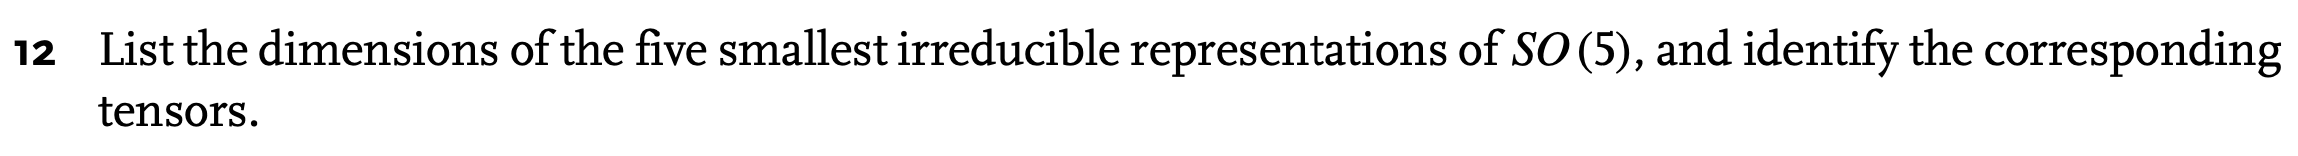
\includegraphics[width=1\textwidth]{IV.1.12.png}
    \end{figure}

    The number of components in an \(k\)-rank tensor furnishing the repr. of \(SO(N)\) is \(N^k\). To have the fewest components, we thus start from the lowest rank.

    The 0-rank tensor (the trivial repr.) is the normalised trace:\begin{align*}
        S^{kk} \to S^{kk}   
    \end{align*}
    It has a dimension of 1.

    Going to 1-rank tensors (vectors), we know that they furnish the defining repr. with \(\dim = 5\).

    Goint to 2-rank tensors, we know we can use the identity to split them into a \(\frac{1}{2} N(N - 1)\) dimensional antisymmetric part, a \(\frac{1}{2} N(N + 1) - 1\) dimensional symmetric part and finally the trace (which we have already counted!). We thus get a \(\dim = 10\) and a \(\dim = 14\) dimensional repr.
    
    We now go to 3-rank tensors. What 3-rank irreducible tensor has the lowest dimensionality (apart from trace)? 
    
    Conraction with the Levi-Civita symbol (dualisation) throws out all the symmetrical parts of a tensor (which is also the trace). Thus, the remaining free components must be totally antisymmetric - and as we have seen, a totally antisymmetric tensor transforms into itself (and therefore constitutes an irreducible repr.). We dualise the three-rank tensor:
    \begin{align*}
        \epsilon^{ijklm} T^{ijk} = \tilde{T}^{lm}
    \end{align*}
    As the dualised vector is a total antisymmetric 2-rank tensor, we have already taken this irrep. into account in fact, just like we have already counted the trace.

    But we can try to count the independent components of the totally symmetric 3-rank tensor. Let's consider an \(j\)-rank tensor in \(SO(5)\). Since it is totally symmetric, we can always order the indicies like \begin{align*}
        S^{55\dots 544\dots 433\dots 322\dots 211\dots 1}
    \end{align*}

    But suppose we we're in \(SO(2)\). Then just by counting how many 2's we had placed, we would know how many 1's we had to place as well (it has to be of rank \(j\)). Once again, since the tensor is totally symmetric, the exact placement of any 2's or 1's doesn't matter, only the count! The possibilites in this case are manageable: We can either have zero 2's, one 2's, two 2's, etc. all the way up to \(j\). This gives \(j + 1\) different symmetric components: \begin{align*}
        \sum_{n_2 = 0}^j 1 = j + 1 
    \end{align*}
    Now we go to \(SO(3)\) (we allow the indicies to run to three). Again, we can use the "canonical ordering" shown above, and we essentially just get a lot of cases of a problem we know how to solve: \begin{itemize}
        \item If there are zero 3's, then we have the exact same problem and we get \(j + 1\)  
        \item If there is one 3, then we count as before, but now there are only \(j - 1\) components left to count with.
        \item If there are two 3's, then we count as before but only with \(j - 2\) components left.
        \item If there are \(n_3\) 3's, then we can count as before but with only \(j - n_3\) components left.
        \item This can go on all the way up to us having \(n_3 = j\) 3's, where there is only 1 possibility.  
    \end{itemize}

    For each of these cases, we get a certain amount of possible distributions of 1's, 2's and 3's. And we want to add them, since we want the total number of such possible distributions, since they correspond to the independent components in the totally symmetric tensor. This is because the distribution has to differ, since ordering doesn't matter. We can thus write \begin{align*}
        \sum_{n_3 = 0}^j \left( \sum_{n_2 = 0} ^{j - n_3} 1 \right) = \sum_{n_3 = 0}^j\sum_{n_2 = 0} ^{j - n_3} 1
    \end{align*}

    This recursive idea of the problem reducing to one we know how to account for but with a different outset (\(j - n_3\) "total" components left for example) is really powerful, and it clearly just generalises to \(SO(5)\). We can thus count the total number of independent symmetric components in a \(j\)-rank tensor in \(SO(5)\) with the sum:
    \begin{align*}
        \sum_{n_5 = 0}^{j} \left(\sum_{n_4 = 0}^{j - n_5} \left(\sum_{n_3 = 0}^{j - n_5 - n_4} \left(\sum_{n_2 = 0}^{j - n_5 - n_4 - n_3} 1 \right)\right)\right)
    \end{align*} 
    (the parantheses are for readibility of the upper limits). This sum can be computed explicitly, but it takes a while by hand. Evaluating with WolframAlpha, we get 35. 

    The final answer is thus: \begin{itemize}
        \item 1 (trace, rank 0)
        \item 5 (defining, rank 1)
        \item 10 (antisymmetric, rank 2)
        \item 14 (symmetric, rank 2)
        \item 35 (symmetric, rank 3)
    \end{itemize}

    In doing this exercise, August first accidently thought we had to solve it for \(SO(4)\). We then got the sum \begin{align*}
        \sum_{n = 0}^j n^{2}  
    \end{align*} 
    and we wanted to evaluate it. It is easiest to prove closed formulas by induction, but then one needs the induction hypothesis. But here is a another powerful approach, in which you study the partial sums as a function: \begin{align*}
        f(n + 1) = f(n) + (n + 1)^{2} = f(n) + n^{2} + 2n + 1
    \end{align*} 
    If one can then match the function at the beginning step, then by induction they must be the same, since for every step, the sum and the function increase by the same amount and thus continue being equal so to say.

    August noticed that 3'rd degree polynomials in \(n\) would have the property that they "spit out" a second degree polynomium: \begin{align*}
        f(n + 1) \stackrel{?}{=} a(n + 1)^3 + b(n + 1)^2 + c(n + 1) = \underbrace{an^3 + bn^{2} + cn}_{f(n)} + a(3n^{2} + 3n + 1) + b(2n + 1) + c
    \end{align*}

    We thus get an equation for the remainder (matching like terms): \begin{align*}
        n^{2} + 2n + 1 = a(3n^{2} + 3n + 1) + b(2n + 1) + c &= 3an ^{2} + (3a + 2b)n + a + b + c\\
        &\implies a = \frac{2}{6}, b = \frac{3}{6}, c = \frac{1}{6}
    \end{align*}
    such that \begin{align*}
        f(n) = \frac{2n^3 + 3n^2 + n}{6} = \frac{n(2n^2 + 3n + 1)}{6}
    \end{align*}
    Also, remember polynomium division: \begin{align*}
        2n^{2}= (n+1) \frac{2n^{2}}{n + 1} = (n + 1) \left(\frac{2(n + 1)^{2} }{n + 1} - \frac{2(n + 1)^{2} - 2n^{2} }{n + 1}\right) = (n + 1) \left( 2n + 2 - \frac{4n + 2}{n + 1} \right)  
    \end{align*}
    such that \begin{align*}
        \frac{n(2n^2 + 3n + 1)}{6} = \frac{n(n + 1) \left( 2n + 2 - \frac{4n + 2}{n + 1} + \frac{3n + 1}{n + 1} \right)  }{6} = \frac{n (n + 1) \left( 2n + 1\right) }{6}
    \end{align*}
    which is in fact the correct form for the sum \begin{align*}
        \sum_{k = 0}^n k^{2} = \frac{1}{6}n(n+1)(2n + 1) 
    \end{align*}

    \begin{figure}[H]
        \centering
        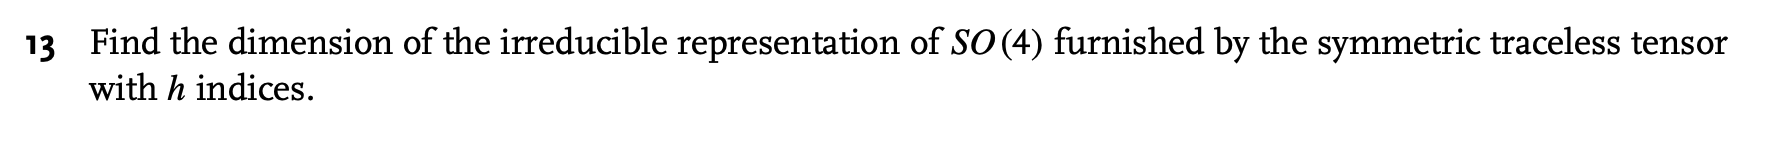
\includegraphics[width=1\textwidth]{figs/IV.1.13.png}
    \end{figure}

\end{document}



\end{document}